\documentclass[letter,12pt]{article}
\usepackage[paperheight=27.94cm,paperwidth=21.59cm,bindingoffset=0in,left=3cm,right=2.0cm, top=3.5cm,bottom=2.5cm, headheight=200pt, headsep=1.0\baselineskip]{geometry}
\usepackage{graphicx,lastpage}
\usepackage{upgreek}
\usepackage{censor}
\usepackage[spanish,es-tabla]{babel}
\usepackage{pdfpages}
\usepackage{tabularx}
\usepackage{graphicx}
\usepackage{adjustbox}
\usepackage{xcolor}
\usepackage{colortbl}
\usepackage{rotating}
\usepackage{multirow}
\usepackage[utf8]{inputenc}
\usepackage{float}

\renewcommand{\tablename}{Tabla}
\usepackage{fancyhdr}
\pagestyle{fancy}


%
\begin{document}
%
   \title{\Huge{Informe Laboratorio 1}}

   \author{\textbf{Sección 1} \\  \\Luis Reyes \\ e-mail: luis.reyes_h@mail.udp.cl}
          
   \date{Abril de 2025}

   \maketitle
   
   \tableofcontents
 
  \newpage
  

\section{Descripción}

\begin{enumerate}
    \item  Usted empieza a trabajar en una empresa tecnológica que se jacta de poseer sistemas que permiten identificar filtraciones de información a través de Deep Packet Inspection (DPI).
    A usted le han encomendado auditar si efectivamente estos sistemas son capaces de detectar las filtraciones a través de tráfico de red. Debido a que el programa ping es ampliamente utilizado desde dentro y hacia fuera de la empresa, su tarea será crear un software que permita replicar tráfico generado por el programa ping con su configuración por defecto, pero con fragmentos de información confidencial. Recuerde que al comparar tráfico real con el generado no debe gatillar alarmas.
    De todas formas, deberá hacer una prueba de concepto, en la cual se demuestre que al conocer el algoritmo, será fácil determinar el mensaje en claro.
    Para los pasos 1,2,3 indicar el texto entregado a IA Generativa y validar si el código resultante cumple con lo requerido.


\end{enumerate}


\section{Actividades}


\subsection{Algoritmo de cifrado}

\begin{enumerate}
\item Generar un programa, en python3 utilizando IA Generativa, que permita cifrar texto utilizando el algoritmo Cesar. Como parámetros de su programa deberá ingresar el string a cifrar y luego el desplazamiento.
\begin{figure}[H]
        \centering
        \includegraphics[width=15cm]{actividades/A1.png}
        \label{fig:a1}
\end{figure}


\end{enumerate}

\subsection{Modo stealth}

\begin{enumerate}
    \item Generar un programa, en python3 utilizando IA Generativa, que permita enviar los caracteres del string (el del paso 1) en varios paquetes ICMP request (un caracter por paquete en el campo data de ICMP) para de esta forma no gatillar sospechas sobre la filtración de datos.
Deberá mostrar los campos de un ping real previo y posterior al suyo y demostrar que su tráfico consideró todos los aspectos para pasar desapercibido.
    \begin{figure}[H]
        \centering
        \includegraphics[width=15cm]{actividades/A2.1.png}
        \label{fig:a2-1}
    \end{figure}
    El último carácter del mensaje se transmite como una b.
    \begin{figure}[H]
            \centering
            \includegraphics[width=15cm]{actividades/A2.2.png}
            \label{fig:a2-2}
        \end{figure}
\end{enumerate}

\subsection{MitM}
\begin{enumerate}
    \item Generar un programa, en python3 utilizando IA Generativa, que permita obtener el mensaje transmitido en el paso2. Como no se sabe cual es el desplazamiento utilizado, genere todas las combinaciones posibles e imprímalas, indicando en verde la opción más probable de ser el mensaje en claro.
    \begin{figure}[H]
        \centering
        \includegraphics[width=12cm]{actividades/A3.png}
        \label{fig:a3}
    \end{figure}
    Finalmente, deberá indicar por que eligió esa IA Generativa en relación a otras del mercado. Comente si tuvo algún problema al momento de generar los códigos.

\end{enumerate}

\section{Desarrollo de Actividades}

\subsection{Actividad 1}
Para esta actividad, se solicita realizar un algoritmo de cifrado utilizando IA generativa. En este caso, se utiliza chatGPT para realizar el código
\begin{figure}[H]
    \centering
    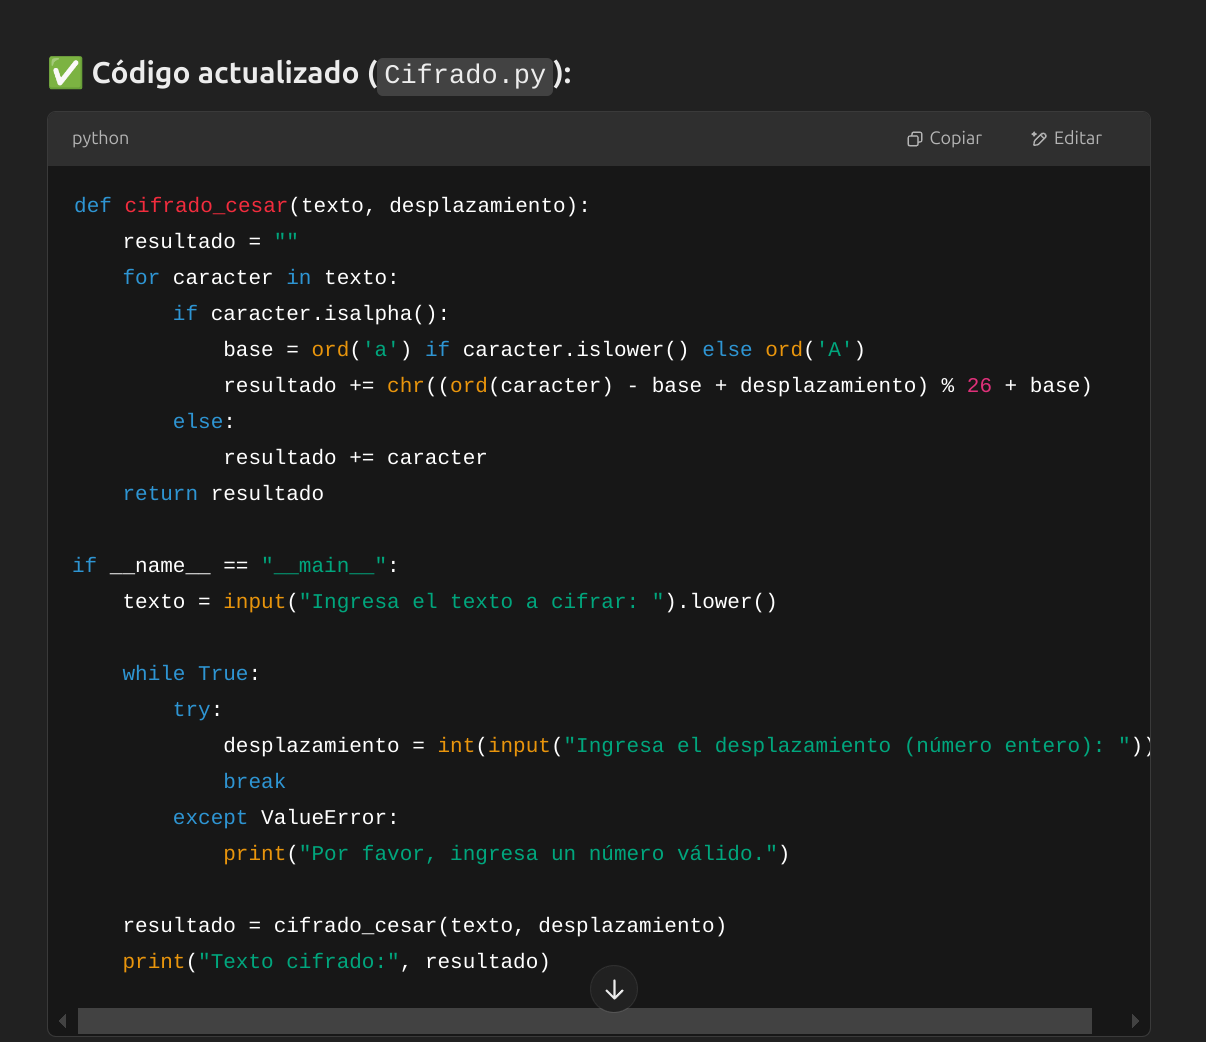
\includegraphics[width=0.8\linewidth]{actividades/Cifrado Cesar.png}
    \caption{Cifrado César generado con IA}
    \label{fig:cifrado-chatgpt}
\end{figure}

El código utilizado tuvo que ser recorregido un par de veces puesto que la IA generaba código incompleto (en primera instancia, no hacía nada, luego no se incluía ni el ingreso de texto por consola ni la salida)
\begin{figure} [H]
    \centering
    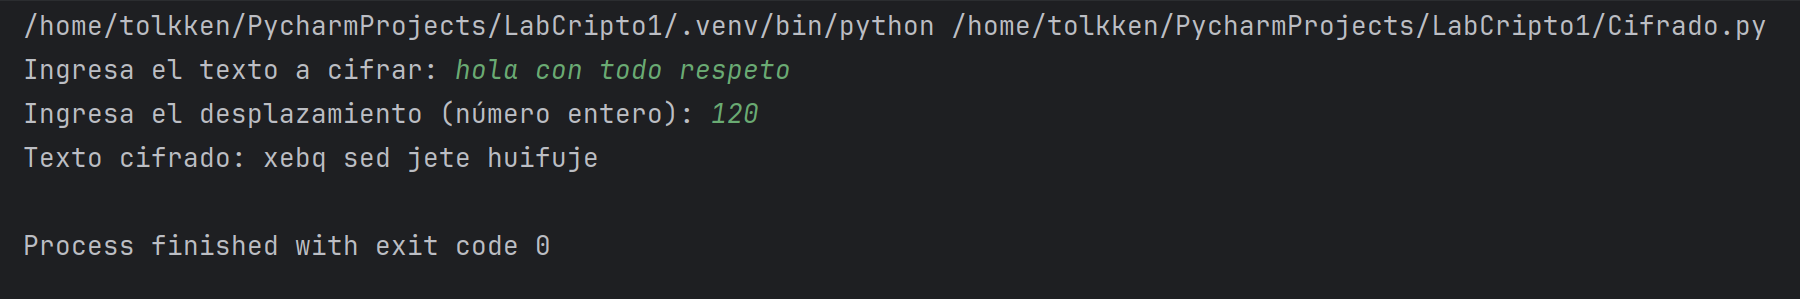
\includegraphics[width=0.75\linewidth]{actividades/Ejemplo de cesar.png}
    \caption{Ejecución del código de cifrado }
    \label{fig:enter-label}
\end{figure}
Se puede observar que el algoritmo funciona incluso con un desplazamiento fuera del rango de 26.
\subsection{Actividad 2}
Para esta actividad, se solicita generar un programa con IA que permita enviar los paquetes generados por el código de la actividad 1 en varios paquetes ICMP request. A modo de no gatillar sospechas, se optó por enviar los paquetes con un pequeño delay (de 0.3 a 3 segundos). De esta manera, no se genera una alarma en el firewall de destino, pues si llegan todos juntos en menos de un segundo, sería un comportamiento bastante sospechoso.
\begin{figure} [H]
    \centering
    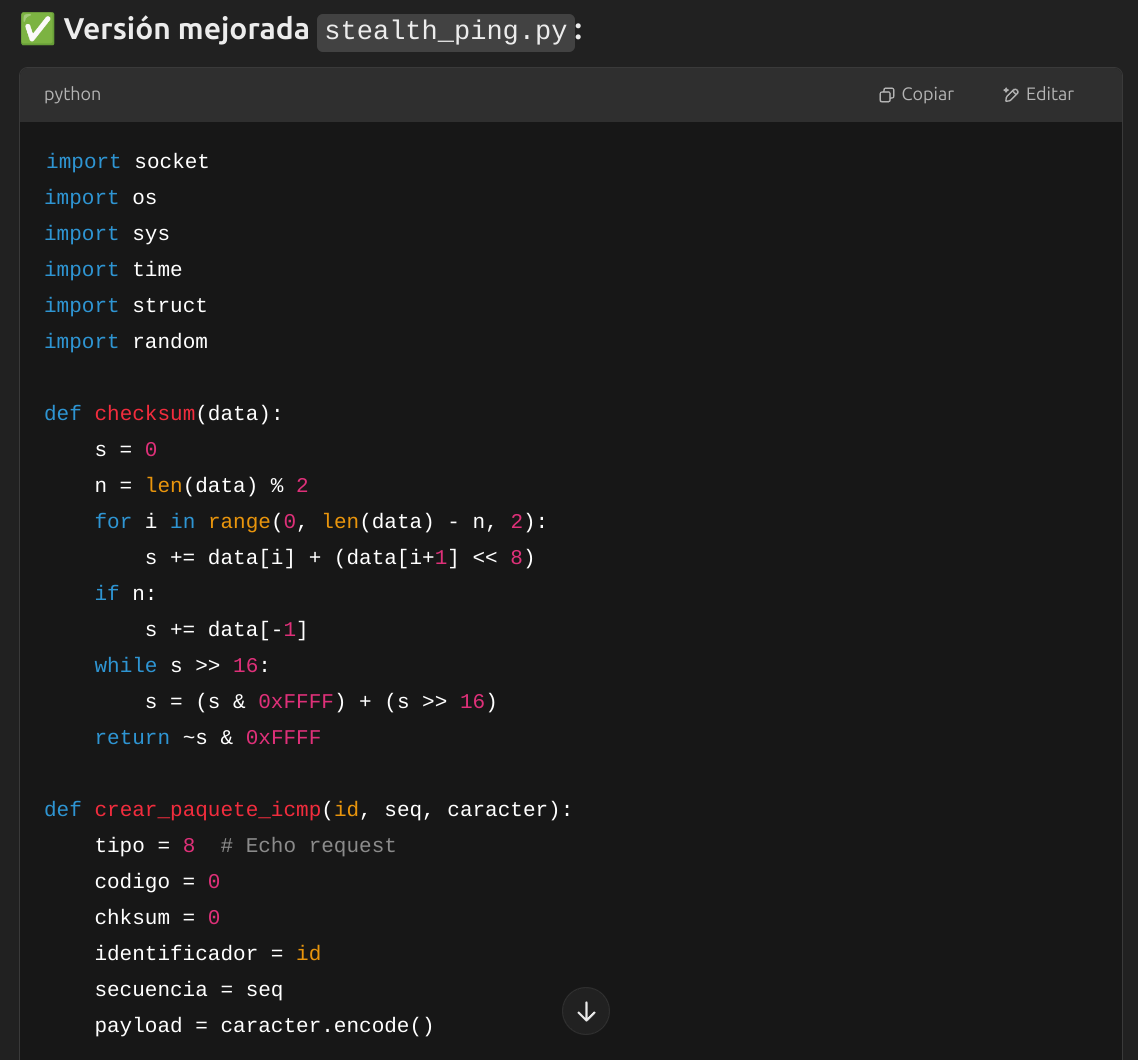
\includegraphics[width=0.7\linewidth]{actividades/Prompt mejorado Stealth.png}
    \caption{Fragmento del código stealth}
    \label{fig:enter-label}
\end{figure}

\begin{figure} [H]
    \centering
    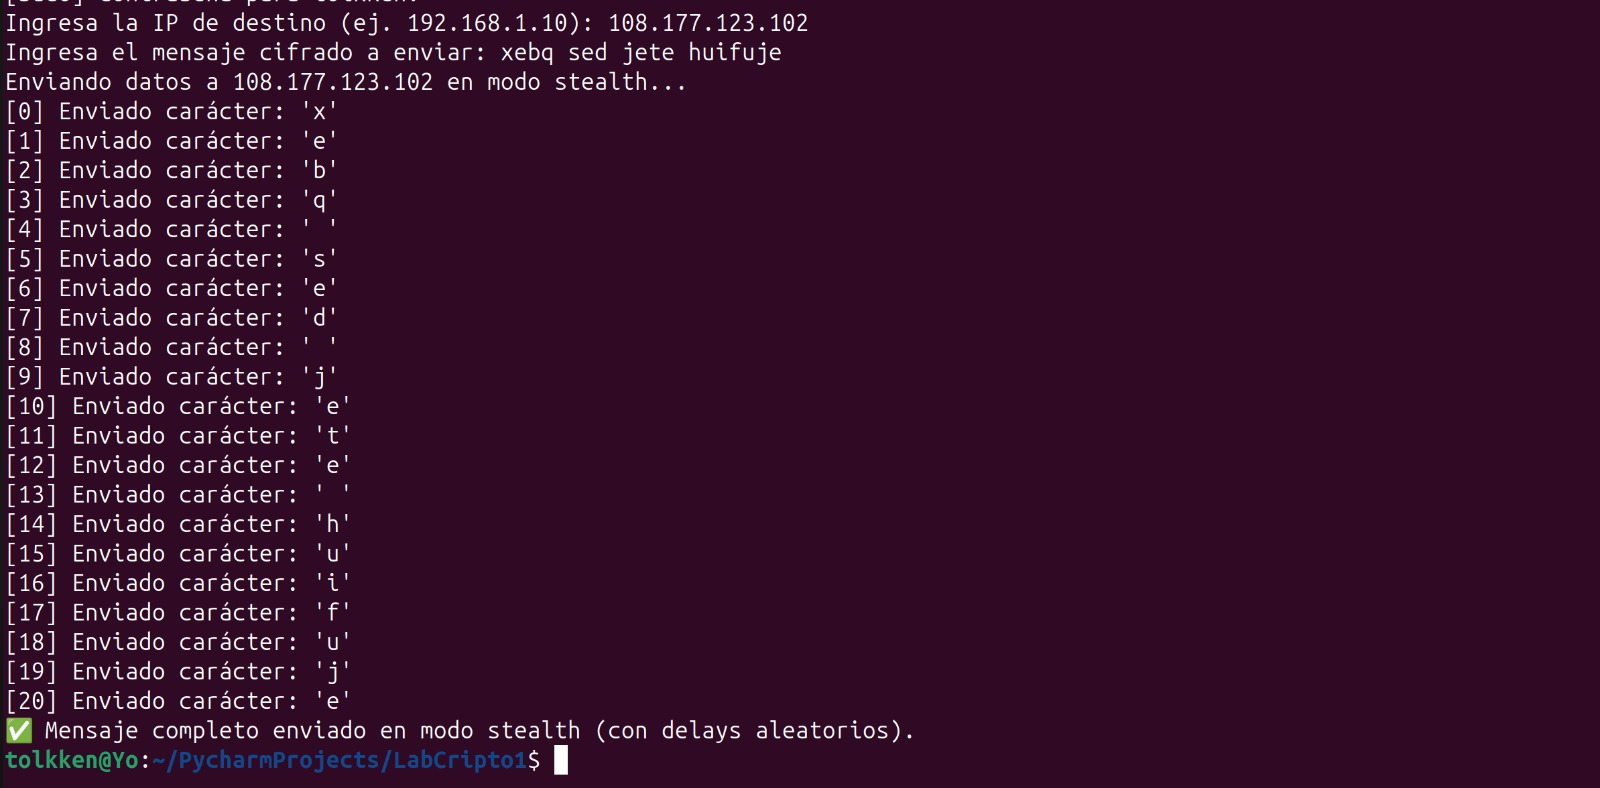
\includegraphics[width=1\linewidth]{actividades/Ejecucion Stealth.png}
    \caption{Ejecucion código stealth}
    \label{fig:enter-label}
\end{figure}

Se puede observar el comportamiento del código de enviar uno por uno los paquetes. Además, los delay aleatorios son observables en los tiempos capturados por wireshark
\begin{figure} [H]
    \centering
    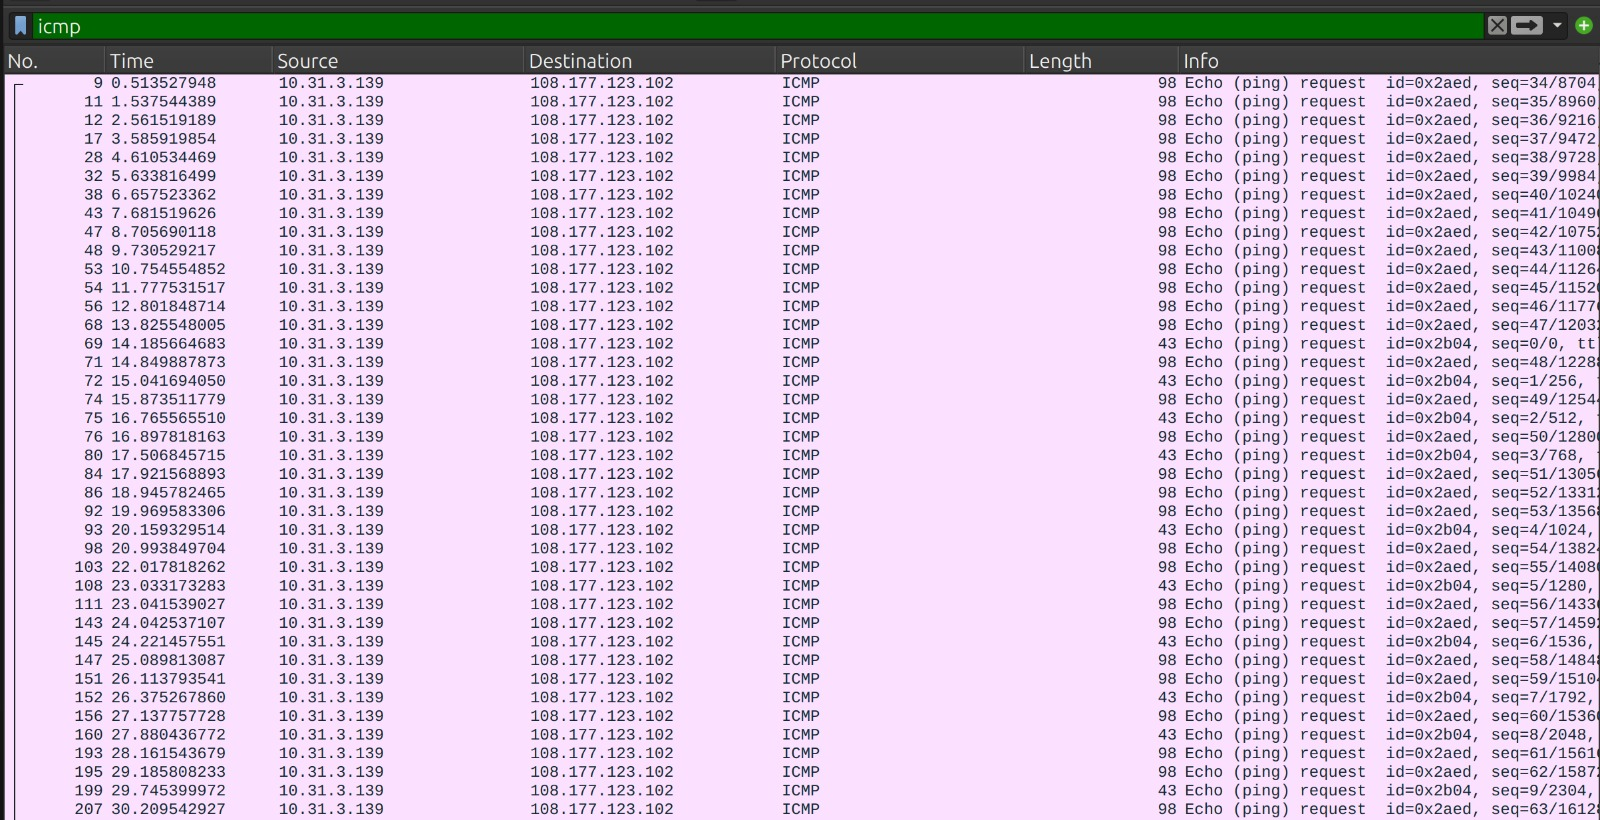
\includegraphics[width=1\linewidth]{actividades/Captura ICMP completa.png}
    \caption{Captura ICMP de un ping a google.com}
    \label{fig:enter-label}
\end{figure}
\begin{figure} [H]
    \centering
    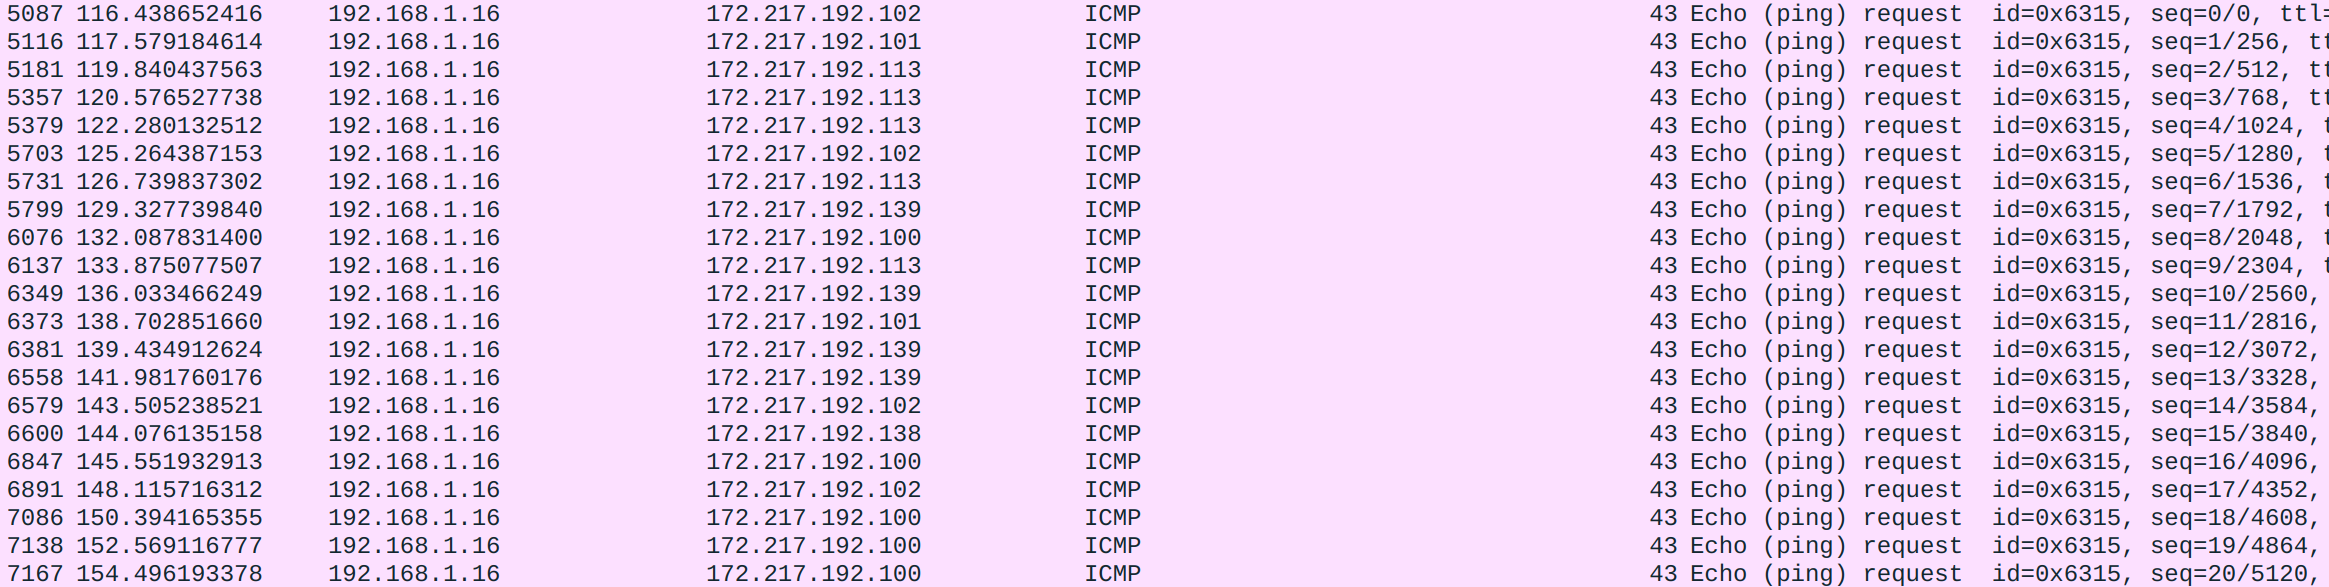
\includegraphics[width=1\linewidth]{actividades/ICMP Wireshark.png}
    \caption{Captura ICMP del algoritmo}
    \label{fig:enter-label}
\end{figure}

Es observable que hay diferencias de máximo 3 segundos entre paquetes, lo que demuestra el correcto funcionamiento del delay del algoritmo
\subsection{Actividad 3}
En esta actividad, se solicita que el mensaje enviado en la actividad 2 se reciba y se desencripte sin conocer el desplazamiento utilizado. Para esto, se imprimen todas las posibles combinaciones destacando el mensaje más probable de ser el real.
\begin{figure} [H]
    \centering
    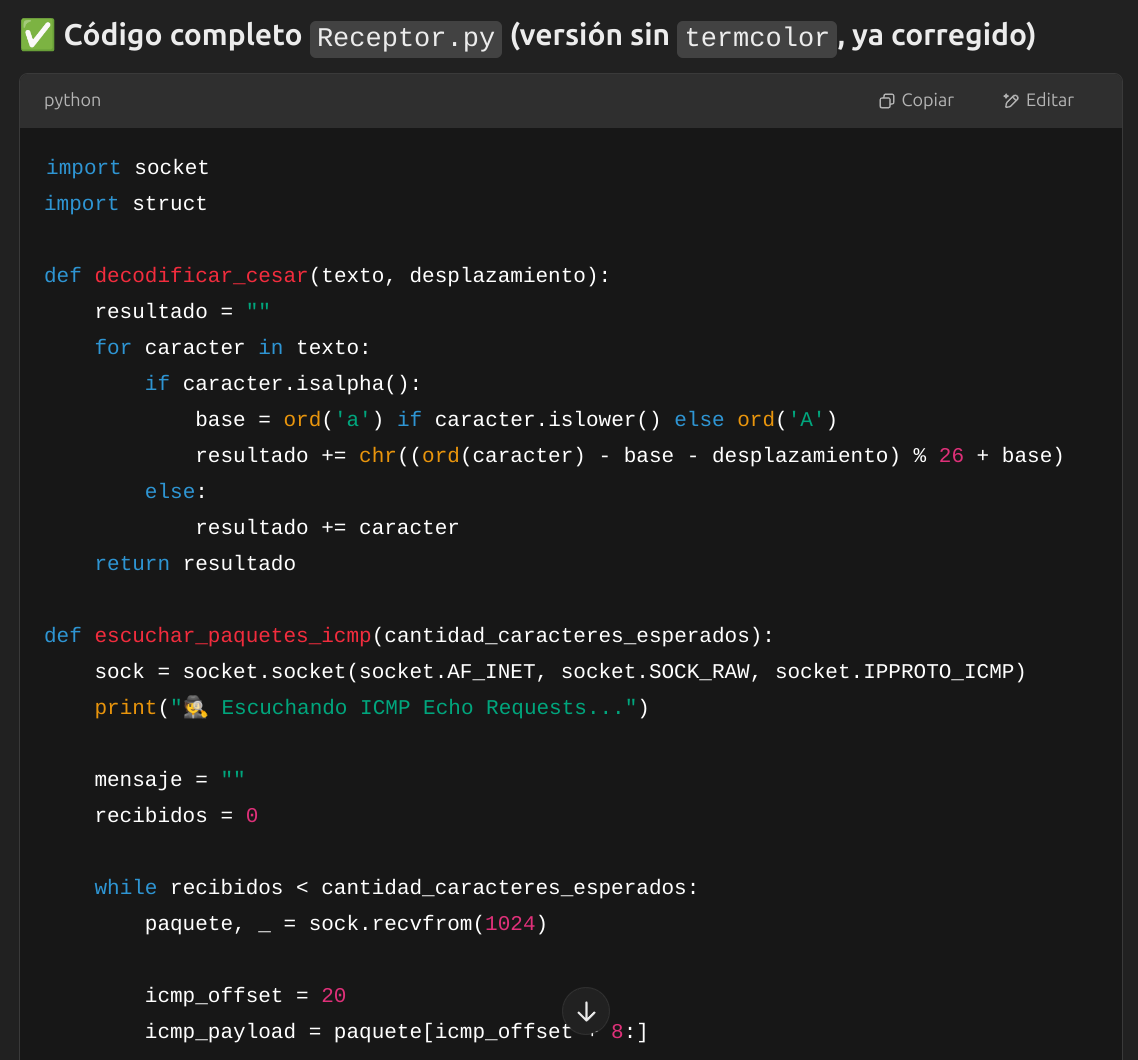
\includegraphics[width=1\linewidth]{Actividad 3/Prompt 3.png}
    \caption{Código MitM}
    \label{fig:enter-label}
\end{figure}
Para este paso, fue necesario rehacer numerosas veces el código por un fallo con la librería termcolor y otros ajustes extras del algoritmo que fallaban (como lo fueron la ip utilizada y el nulo trabajo del receptor). Finalmente, dado que al realizar un ping no hay respuesta por parte del receptor, se utilizó localhost para capturar directamente los paquetes enviados.
\begin{figure} [H]
    \centering
    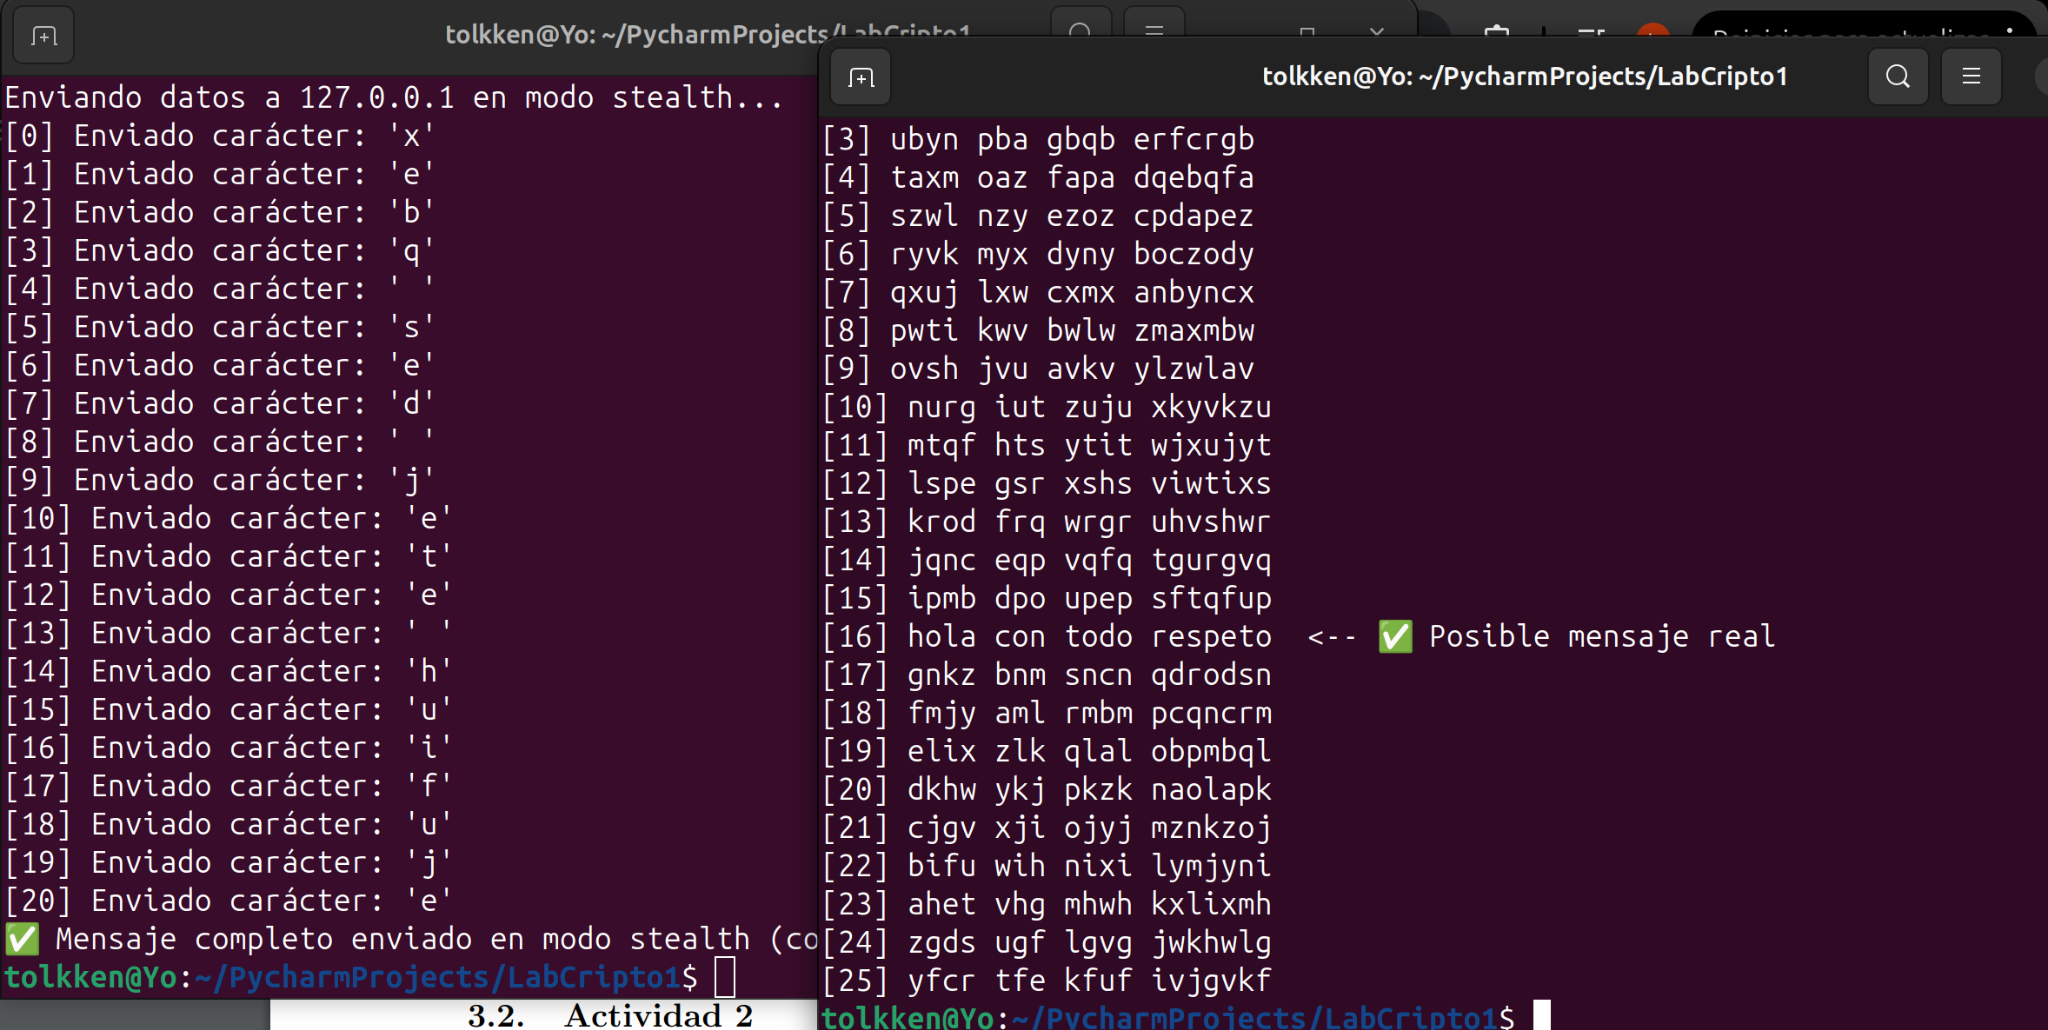
\includegraphics[width=1\linewidth]{Actividad 3/Ejecucion mitM.png}
    \caption{Ejecucion codigo MitM}
    \label{fig:enter-label}
\end{figure}

Se puede observar en ambas terminales los códigos de la actividad 2 (stealth) y de la actividad 3 (mitM) funcionando y enviando/recibiendo el mensaje. Asimismo, el algoritmo de desencriptado reconoce claramente el mensaje completo de entre todas las opciones posibles. Esto demuestra un correcto funcionamiento de los distintos algoritmos utilizados para este laboratorio.

Finalmente, mencionar que la preferencia de utilizar chatGPT radica tanto en el hecho de su popularidad y comodidad de uso como en el hecho de tener la versión de pago, lo que me facilita códigos mucho más útiles y eficaces que los de la versión gratuita.


% Please add the following required packages to your document preamble:
%\begin{table}[htbp]

\section*{Conclusiones y comentarios}
El laboratorio completo permitió conocer cómo funcionan los algoritmos básicos de cifrado y de desencriptación, asi como burlar barreras de seguridad evitando enviar todos los paquetes en un mismo instante y optar por enviarlos con un ligero delay. También se pudo observar cómo actúa la IA generativa en la creación de algoritmos de cifrados, mostrando ser una herramienta estupenda para acelerar el trabajo, pero no perfecta, pues los errores que aún comete son necesarios de revisar si no se quiere tener un algoritmo defectuoso 
(o directamente no funcional).
\end{document}
